\hyphenation{ma-te-rials}
%%%%%%%%%%%%%%%%%%%%% Introduction %%%%%%%%%%%%%%%%%
\chapter{Introduction}
\label{ch:intro}


\indent Richard Feynman, a Physics Nobel Prize winner whom I consider one of the brightest physicists who has ever lived on Earth, once summarised in one single phrase what he believed to be the most important fact about the world around us: "all things are made of atoms" \cite{Feynman_atoms}. Feynman himself was the father of the quantum electrodynamics but in this simple statement delivered originally to Caltech students and now known to everyone through his series of physics books, he decided not go into quantum mechanics principles and rather illustrated at the highly abstract level that everything is made of smaller particles. 

Nowadays we know that atoms have heavy nuclei and light electrons "orbiting" around the nucleus on the electron shells. The nucleus is positively charged proportionally to the number of protons it contains. To provide the stability of the nuclei of the heavy atoms our world also needs neutrons, which have no electric charge. %A free neutron decays in about 15 minutes, while the proton is stable, as far as we know from the experiments, and only in some exotic %Beyond the Standard Model (BSM) theories it is hypothesised that the proton lifetime is finite. However, the estimate of the proton lifetime is a value that is larger than the age of our Universe and is at least $10^{30}$ years \cite{DIMOPOULOS1982133}. 
Going further to an even smaller scale, we now know that protons and neutrons are not elementary, instead they are composed of point-like constituents that are called quarks (see Figure \ref{atom_structure}). 

\begin{figure}[H]
  \centering
    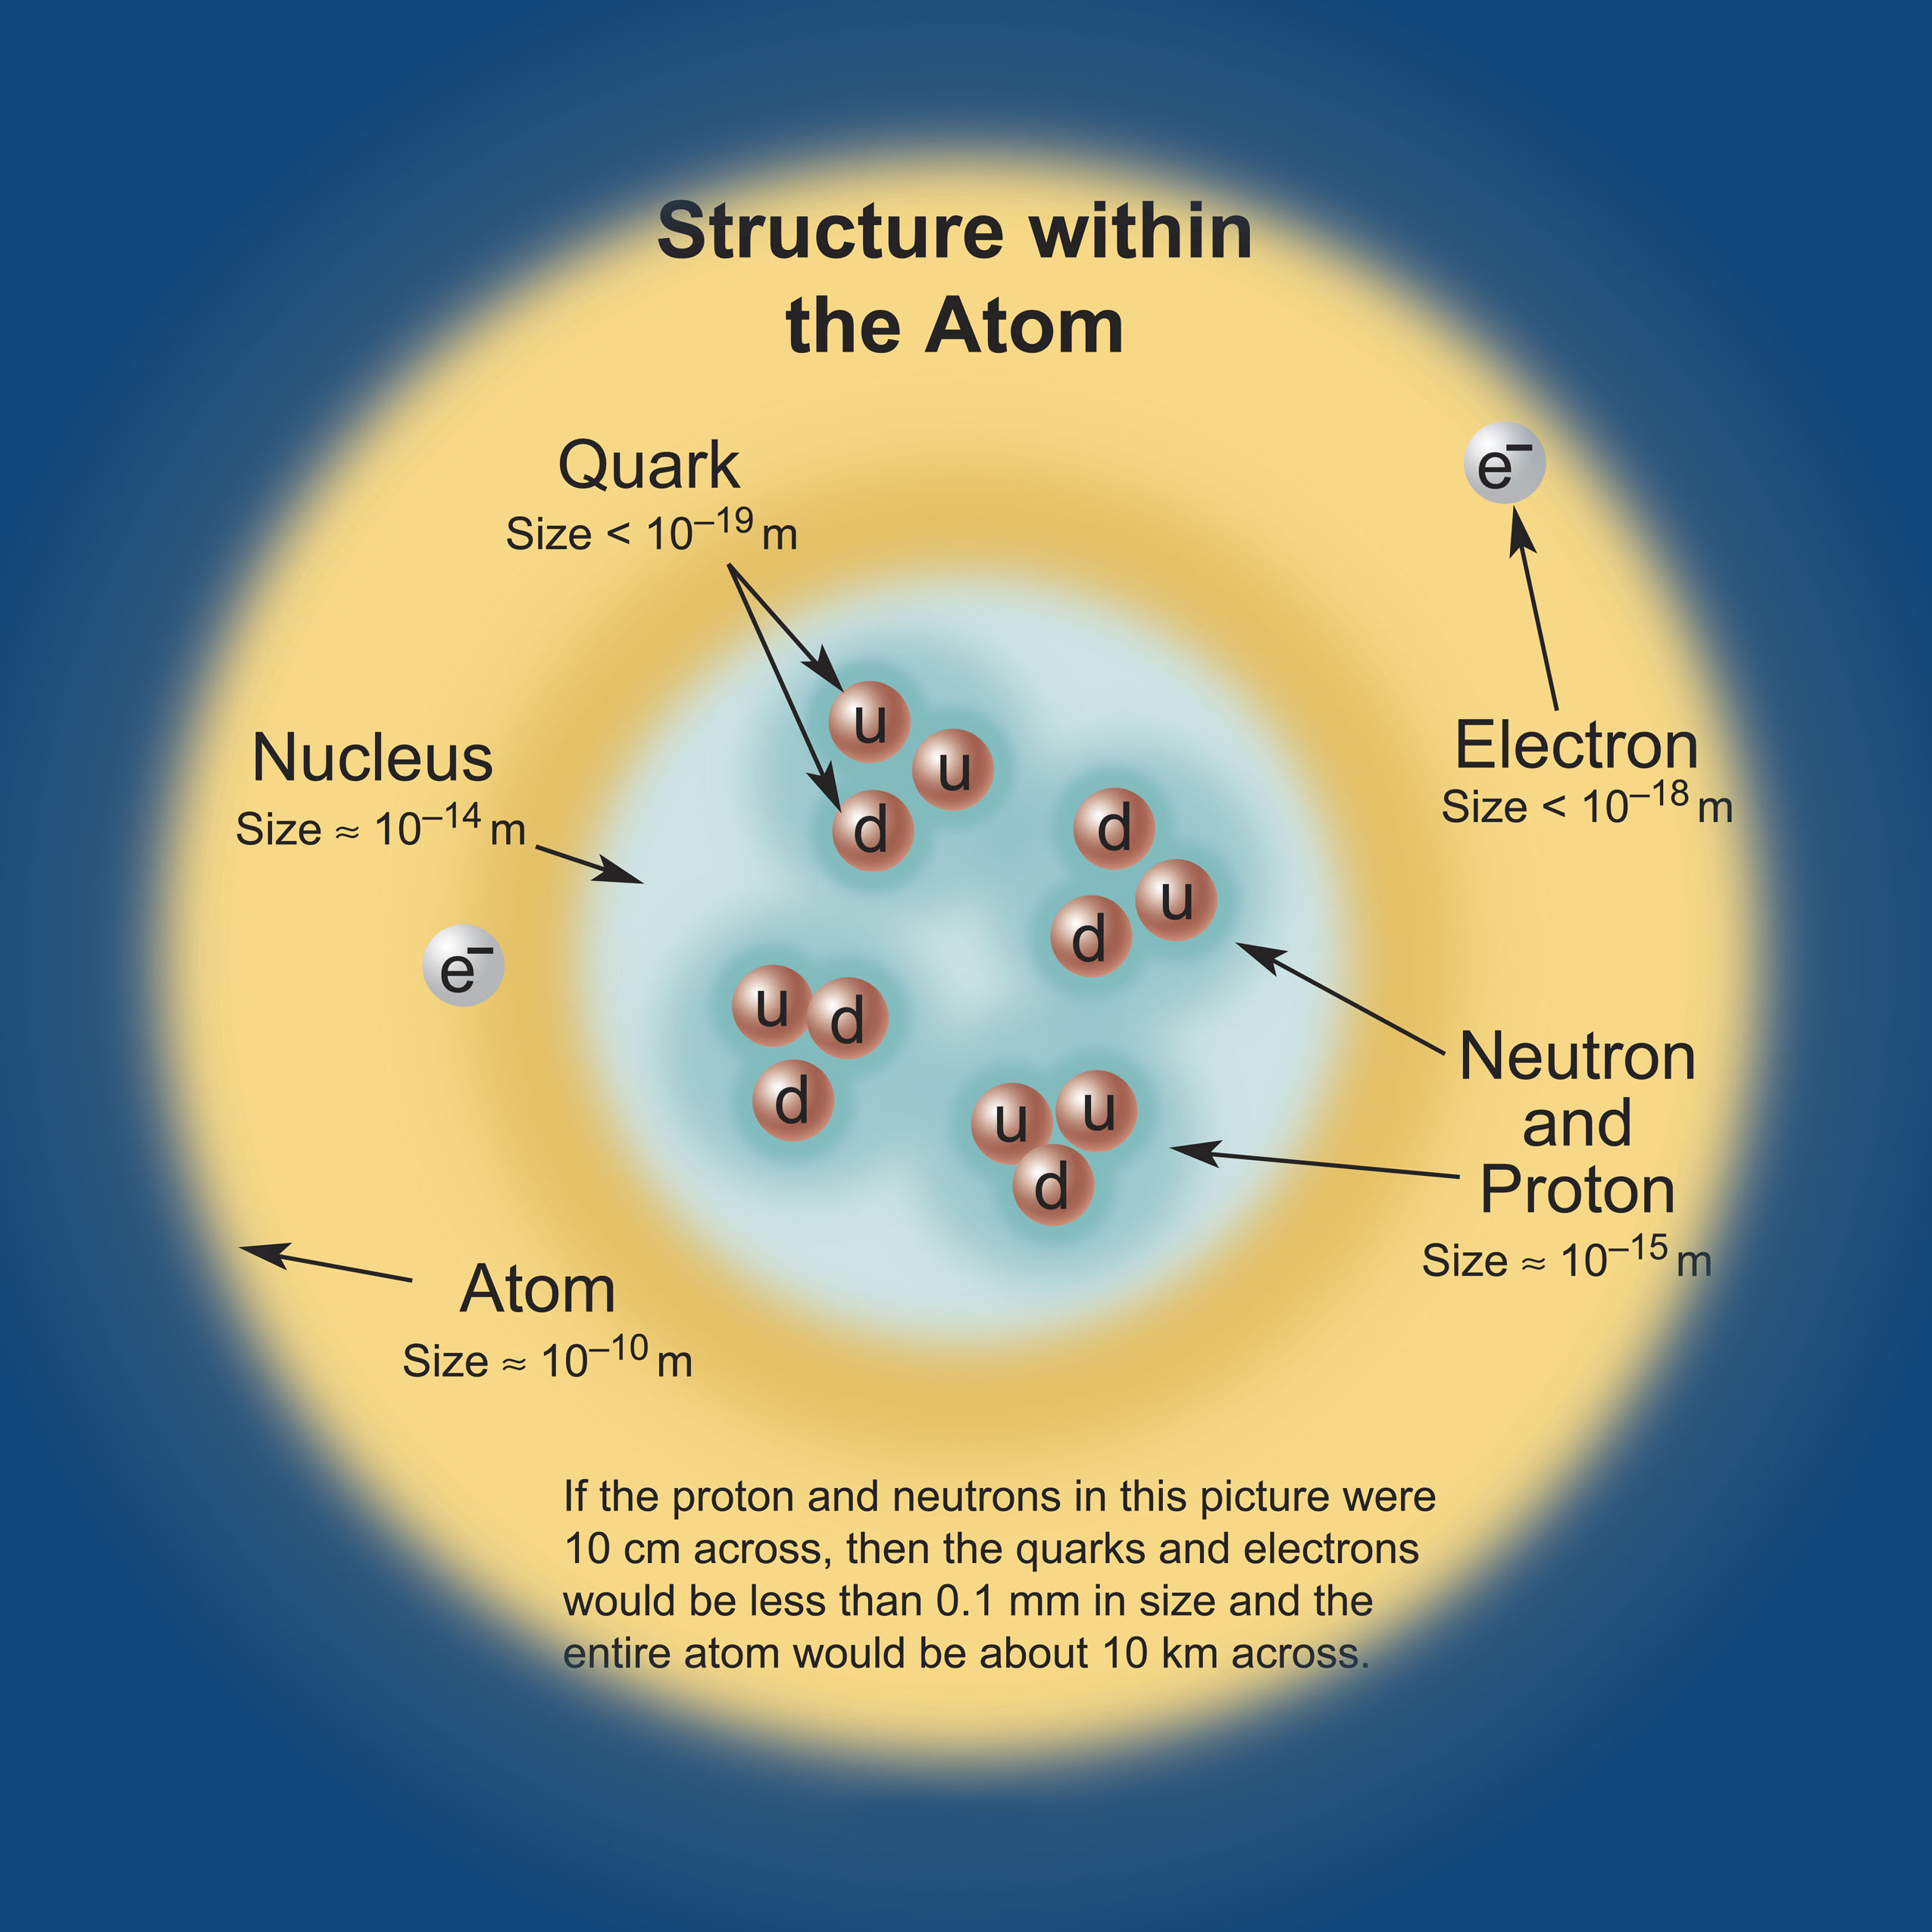
\includegraphics[width=0.70\textwidth]{atom_structure}
    \caption[The structure of an atom]{The structure of an atom. Approximate scale values are indicated.}
    \label{atom_structure}
\end{figure}

Quarks were proposed by Gell-Mann and also by Zweig to explain periodicity in properties of observed subatomic particles.  \cite{griffiths_hep}. Quarks come in three families, or generations, and are arranged into doublets. A doublet  is mathematical construct that is used to explain two-level/value system. For example, by design of Gell-Mann and Zweig, each doublet in their theory is a two quark system that has an "up" quark with the electric charge $-1/3$ and a "down" quark with the charge $+2/3$. For antiquarks signs are reversed. 

Physics world before Gell-Mann and Zweig got used to the fact that particles have integer charges due to enormous number of observations. The fact that the quark charge values were fractional was so revolutionary that Gell-Mann decided not to publish his article in a highly prestigious journal but, expecting a rejection, decided to go with the second tier one \cite{griffiths_hep}. There are six different types of quarks and to distinguish one from another there is a "flavor" number assigned to them. For instance, a charm quark has $+1$ unit of "charmness", while a strange quark has $-1$ unit of "strangeness". All the other quark flavor fields are zero for them. And this pattern is applied to all the other four quarks to fill the corresponding "quarkness" numbers. Besides, the mass of quarks increases from the first to the third family. No explanation exists in the Standard Model (SM). 

SM is the mathematical theory that has been extremely successful describing the interactions of elementary particles and fields. SM includes all known interactions except gravity. For the last several decades SM is the most tested theory of fundamental forces and elementary particles and is presently generally accepted by the whole physics community. Formally, all SM elementary particles are split into two classes: fermions and bosons. Particles with the half-integer spin 1/2 (quarks and leptons) are called fermions since they obey Fermi-Dirac statistics ~\cite{statmech}. The other class of particles is bosons. They are force carriers, have an integer spin, and are characterised by the Bose-Einstein statistics. 


Continuing with quarks, their another important characteristics has been revealed at the $e^+e^-$ colliders when physicists compared production rates of muons and hadrons. The theory was off by a factor of three. This was the motivation to introduce three quark colours: green, blue, and red. Quarks were observed decades after electrons have been discovered. In particle physics, electron belong to a family of leptons. A lepton is an elementary particle with the spin 1/2 that participates in all but strong interactions, which will be discussed in more detail later in this chapter. An electron was discovered by Thompson \cite{Davis:1989898} in 1897 when he was studying the properties of a cathode ray. Due to this discovery, that year may be considered the beginning of an era of a particle physics: a dozen of particles have been discovered in the next decades. In 1936, another lepton was observed, a muon \cite{Piccioni1996}, in an experiment of Anderson and Neddermeyer who studied cosmic radiation. In essence, a muon is almost a copy of an electron, but is 207 times heavier and no explanation for this mass difference exists in the SM. As a side note, according to Carl Bender, there is a story that Feynman was able to derive the mass of the muon starting with the mass of an electron, but the world has never seen that calculation published \cite{Bender}. 



Analogously to quark families, leptons are also arranged in generations. Each generation is a doublet that consists of a charged lepton (electron, muon or tau) with the charge $-1$ and a neutral lepton (corresponding electron, muon, or a tau neutrino). An electron and a muon neutrinos have been discovered in 1956 and 1962, respectively. 
The existence of the electron neutrino was deduced from the violation of the conservation of energy in a beta decay, while the muon neutrino \cite{PhysRevLett.9.36} was discovered by Schwartz, Lederman, and Steinberger during an experiment with the pion beam where leptons from the pion decays arrive to the aluminum spark chamber after passing the steel wall. 51 events of interest have been observed after running the experiment for several months.
Those events could not be due to electron neutrinos, since they will interact with the metal and produce electrons. The presence of narrow muon tracks in the chamber in each event, hence muons, was a clear indication that those neutrinos were of a different kind, they were muon neutrinos. Finally, a tau lepton and a tau neutrino were discovered in 1975 and 2000 correspondingly \cite{PhysRevLett.35.1489, Kodama:2000mp}. With that, all three families of the SM leptons were observed: a long-awaited tau neutrino, which was decades ago theoretically speculated to exist, was finally discovered experimentally. In a like manner to families of quarks, lepton masses grow with the generation, where a tau from the third generation is the heaviest lepton. To classify leptons of different families the lepton numbers have been reserved: 1 unit of electron number to an electron and an electron neutrino, 1 unit of muon number to a muon and an muon neutrino, and 1 unit of tau number to a tau and a tau neutrino.

In the SM there are four fundamental forces: gravitational, weak, electromagnetic, and strong forces. 
%At the fundamental level the world is made of quarks and leptons. And there must be rules, at least we expect them to exist, which explain how quarks/leptons interact. These rules are referred to as fundamental forces of nature. 
We will classify all four forces \cite{wolfram} in terms of the relative strength, the range that they can cover, the spin of the mediator, and whether the force's nature is attractive, repulsive, or both. This should be taken with the grain of salt though, since this is quite ambiguous categorisation, but it has a deep pedagogical meaning because it helps to illustrate in which regime each of the forces is dominant. According to Carl Bender, this is of great importance since it is one of the main approaches to solving physics problems: to know which effects are the dominant and which are sub-dominant. This helps to justify what effect can be neglected and what approximation can be used, thus, allowing the possibility to do calculations for problems where closed-form solutions do not exits, which is almost all the complex phenomena around us \cite{Bender}. 


The first force on our list of SM forces is the the gravitational force. This force governs the Universe at the macroscopic level: planets, solar systems, etc. The first theory of gravity was formulated by Newton \cite{Chandrasekhar:1187874} and then further developed by Einstein. A good historical perspective is available at \cite{Gutfreund:1980674}. It is worth noting that the gravitational force is not included in the SM. Attempts are ongoing to expand the SM, e.g., adding the graviton as a mediator, but no real success so far has been achieved to create a renormalizable theory that would combine both SM and gravity \cite{butterworth2014smashing}. To surprise of many, gravity is the weakest force, the only reason why the motion of planets and galaxies is governed by gravity is because those are gigantic objects. Gravity effects become the dominant ones at the macroscopic scale because of an enormous number of particles involved in the interaction. If the strength of the strongest force, which is the strong force, is set to 1, then the strength of the gravity will be about $10^{-41}$. It is contemplated that the gravity mediator (the graviton), if exists, would have a charge of zero, zero mass, spin 2, and should be a stable particle. The gravitational force is of the infinite range and its nature is purely attractive, while all other three forces can exhibit both an attractive and a repulsive behaviour. Einstein's general relativity theory is the only proven working theory of gravity as of now, though not a quantum theory. %, and sometimes is called "geometrodynamics". 

The next force we are going to discuss is the weak force. It is mediated by a charged W (charge +1/-1) boson or a neutral Z boson, thus giving name to charged and neutral weak interactions correspondingly. All SM fermions experience the weak force, both quarks and leptons. %For leptons, it is worth mentioning here that neutral leptons have no charge, thus will not participate in the electromagnetic interactions, and all leptons have no color charge, so they feel no strong force \cite{griffiths_hep}. 
The relative strength of the weak force is $10^{-16}$ and the range of applicability is $10^{-3}$ fm. All three weak bosons ($W^+$, $W^-$, and Z) have spin 1 and are quite massive: $m_{W^\pm} = 80. 385$ GeV and $m_{Z}=91.189$ GeV. GeV is the unit of the so-called "natural system of units", in which $\hbar = c = 1$. This system is very popular in the high-energy physics and is widely used in this thesis. Adoption of this system simplifies how many equations look and also makes a fine-structure constant $\alpha \approx 1/137$ dimensionless. Using the natural system of units \cite{Cottingham:1026625} masses, momenta, and energies are measured in electronvolts (eV), with GeV ($10^9 $~eV) and TeV ($10^{12}$~eV) being the most popular units in a modern high-energy physics due to energy regimes involved. 



Charged weak interactions are interesting due to the fact that a primitive interaction vertex can be intuitively thought of as a point where a charged lepton is converted to a neutral lepton or vice versa. A good example is a muon decay, which is nothing but a conversion of the muon to a muon neutrino with the help of the W boson, which further decays to an electron and a corresponding electron antineutrino. %Lepton numbers are conserved during weak interactions and conversions happen only within the same family of leptons. However, c
It is worth noting that charged weak interactions do not conserve the flavor of quarks, e.g., members of doublets of the third and the second families can be converted into members of the lower family of quarks. This fact is reflected in the Cabibbo-Kobayashi-Maskawa (CKM) matrix \cite{pdg}. This matrix describes the strength of the flavour-changing weak interactions. Since diagonal elements of this matrix are less than one and off-diagonal elements are non-zero, CKM matrix represents a mismatch of quantum states of quarks when they propagate freely and when they take part in the weak interactions. In other words, the CKM matrix with non-zero off-diagonal elements means cross-generation interactions are allowed and this is the information that the CKM matrix quantifies.

\begin{equation}
\small
\begin{pmatrix}
|V_{ud}| & |V_{us}| & |V_{ub}| \\
|V_{cd}| & |V_{cs}| & |V_{cb}| \\
|V_{td}| & |V_{ts}| & |V_{tb}|
\end{pmatrix} = \begin{pmatrix}
0.97427 \pm 0.00015 & 0.22534 \pm 0.00065 & 0.00351^{+0.00015}_{-0.00014} \\
0.22520 \pm 0.00065 & 0.97344 \pm 0.00016 & 0.0412^{+0.0011}_{-0.0005} \\
0.00867^{+0.00029}_{-0.00031} & 0.0404^{+0.0011}_{-0.0005} & 0.999146^{+0.000021}_{-0.000046}
\end{pmatrix}.
\label{eq:ckm}
\end{equation}


In SM several multi-boson vertices are allowed. W and Z bosons that mediate weak interactions can couple to each other, so $WWZ, WWWW$, and $WWZZ$ vertices are possible in the SM. In addition, W boson that participates in charged weak interactions also couples to photons, so $\gamma WW$, $\gamma WWZ$, and $WW\gamma\gamma$ vertices are also allowed.

Now, we are moving to the electromagnetic (EM) force. This is one of the main forces that we experience in our everyday life. The reason the reader can sit in the chair and do not fall further down due to gravity, is that electrons of the reader's body repel electrons of the chair. Relative strength of the EM force is $10^{-3}$ and the range of applicability is infinite. A photon, as its mediator, has zero mass, spin 1, and the theory that describes its interaction with leptons and quarks is called quantum electrodynamics (QED), developed in 1940th and 1950th by Tomonaga, Schwinger, Feynman, and Dyson \cite{qed_fathers}. Electric charge is conserved in EM interactions and no single photon-to-fermion vertex is possible, there are always two fermions that must be involved.% in such a way that their net electric charge is zero. 
Lastly, even though Z boson is massive and photon is massless, Z boson is neutral, thus, any interaction where the photon is a force carrier, can be also mediated by the Z boson.


Finally, we can talk about the forth force of the SM - the strong force. This is the strongest known force and the gluons are the carriers. There are nine types of gluons and each gluon carries one unit of color and one unit of anticolor. But, technically, the ninth gluon is a color invariant, and would give rise to an infinite range of the strong force, which contradicts experiments. That is why modern physics assumes that in our world only eight gluons exist \cite{griffiths_hep, pdg}. Gluons carry color charge and can couple to each other. For several high order processes in quantum chromodynamics (QCD), 3- and 4-gluon vertices have to be introduced to restore gauge invariance and no higher order vertices are required \cite{Mangano:454171}.
 

We can summarise the knowledge about four fundamental forces in one figure using the Feynman diagram representation \cite{feynman_diagrams}. Fig. \ref{SM_vertices} shows all allowed SM particle interactions and corresponding simple vertices.
	
\begin{figure}[H]
  \centering
    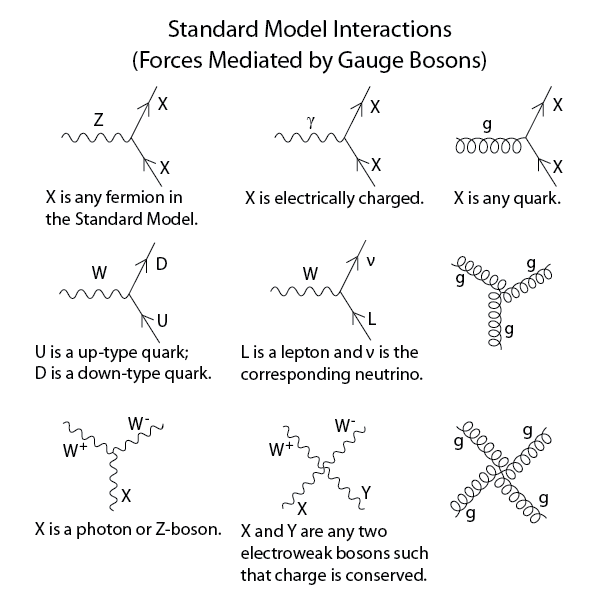
\includegraphics[width=0.80\textwidth]{Standard_Model_Feynman_Diagram_Vertices}
    \caption[All SM interaction and simple vertices]{All SM interaction and simple vertices. }
    \label{SM_vertices}
\end{figure}



	
The description of the SM picture will not be complete without mentioning the main particle, yet missing until 2012$^{th}$ ... the Higgs boson! (Fig. \ref{sm_interactions2} \cite{strassler}) After the electroweak (EW) unification by Glashow, Salam, and Weinberg \cite{Glashow:1961tr}, it was still not clear what is the origin of the mass of fundamental particles. In 1964, Robert Brout and Fran�ois Englert\cite{PhysRevLett.13.321}, Peter Higgs\cite{PhysRevLett.13.508}, Gerald Guralnik, C. Richard Hagen, and Tom Kibble \cite{PhysRevLett.13.585} (BEHGHK authors), proposed the method by which the particles can acquire mass. This technique consists of three stages and we will discuss them one-by-one:

\begin{figure}[H]
  \centering
    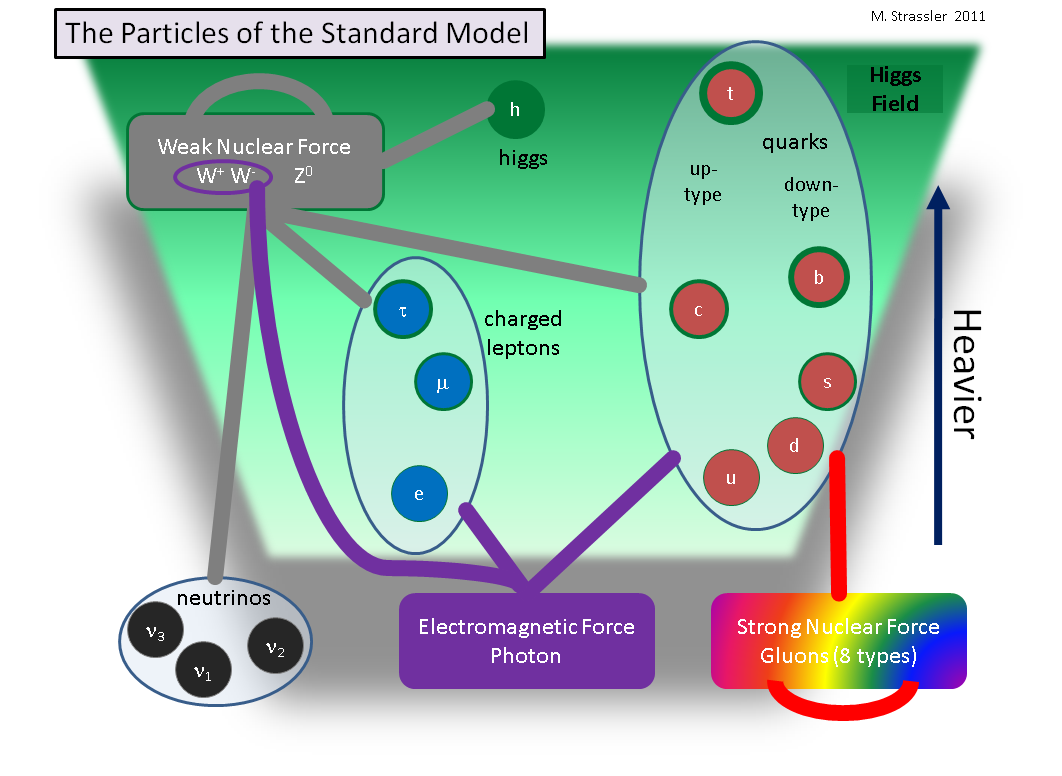
\includegraphics[width=0.80\textwidth]{sm_interactions2}
    \caption[SM particles and force carriers]{SM particles and force carriers. Self-interactions are also shown. The strength of the coupling to the Higgs boson increases from the bottom to the top, which is illustrated by the shades of the green color (the Higgs field).  }
    \label{sm_interactions2}
\end{figure}



\begin{enumerate}
\item The Brout-Englert-Higgs (BEH) mechanism
%\begin{enumerate}
%\item Nested item 1
%\item Nested item 2
%\end{enumerate}
\item The BEH field
\item The Higgs boson.
%\ldots
\end{enumerate}

The first stage, the BEH mechanism, is simply a spontaneous symmetry breaking (SSB) mechanism, which is a mathematical trick consisting of rewriting the original scalar fields in the EW Lagrangian, rearranging equations, and requiring that the fields are real. What does this lead to? We started with a scalar complex field and a massless vector field and after SSB we obtained a single real scalar field (Higgs boson) and a massive vector field. In terms of our physical world this it what gives mass to W and Z bosons. 

The second stage is the BEH field. It exists everywhere and has been present almost since the Big Bang \cite{who_cares}. It is a property of our world. All the fundamental particles that interact with the BEH field acquire mass. Those, who do not interact directly (at the tree level), have no mass and all their energy is in the form of the momentum, thus they can travel with the speed of light. The more the particle interacts with the BEH field, the higher is the coupling to the Higgs boson or simply the higher is the mass of the particle. For example, the coupling of the Higgs boson to fermions is proportional to the mass of the fermions, while for W and Z bosons it is proportional to the squared mass of bosons, thus top quark and Z bosons are quite massive (see Fig. \ref{coupling_ff} \cite{CMS-PAS-HIG-14-009}). 

\begin{figure}[H]
  \centering
    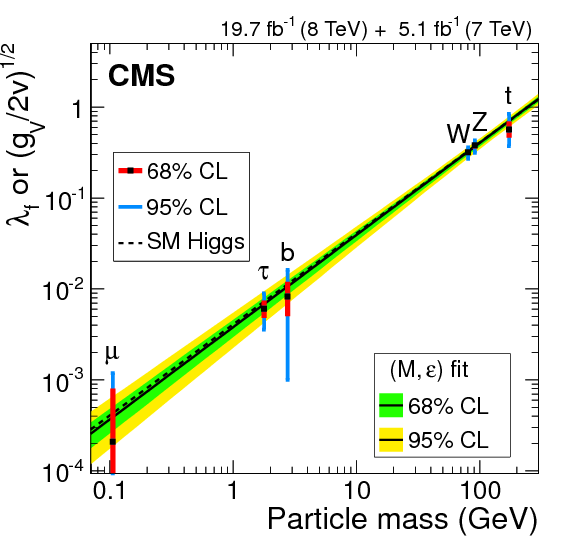
\includegraphics[width=0.80\textwidth]{coupling_ff}
    \caption[Coupling of particles to SM Higgs boson]{Coupling of particles to SM Higgs boson versus the mass of the particle, log-log scale is used.}
    \label{coupling_ff}
\end{figure}



The third and arguably the most important stage - the Higgs boson. The Higgs boson is the excitation of the BEH field. Thus, the Higgs bosons can be produced at colliders by pumping more and more energy in a small space-time region exciting the BEH field to "produce" the Higgs bosons. In reality this happens through making the LHC beams more energetic and thus, during the collision, having more energetic gluons (and also quarks). The main production mechanism is called a gluon fusion, when through the top quark loop a single Higgs boson is produced. This accounts for about $90\%$ of the overall LHC Higgs production at the 13 TeV energy. The second mechanism is a vector boson fusion. The third mechanism is the associated production with a weak boson. And the smallest contributor to the Higgs boson production is the ttH process, which stands for the associated production of the Higgs boson with the top anti-top quark pair.% (see Fig. \ref{higgs_production}). 
All mentioned Higgs boson production mechanisms are presented in the form of Feynman diagrams in Fig. \ref{higgs_production}.

\begin{figure}[H]
  \centering
    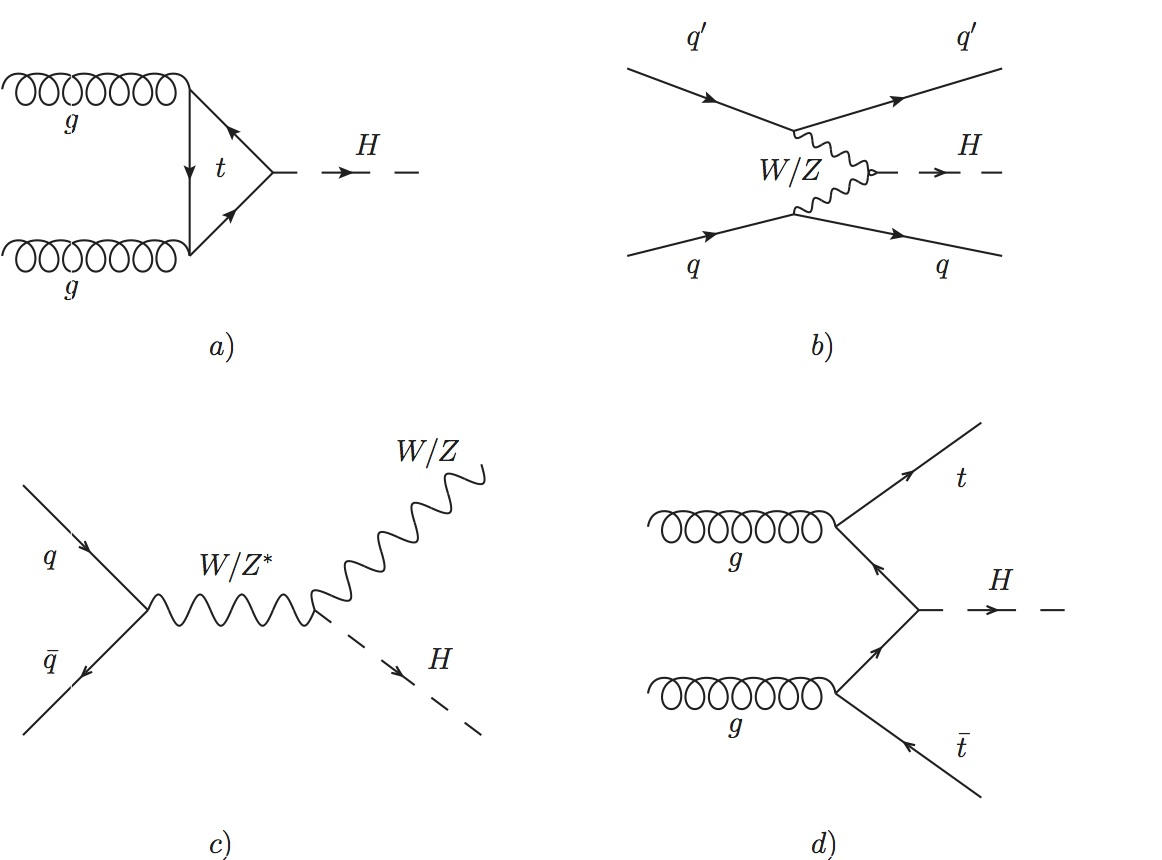
\includegraphics[width=0.80\textwidth]{higgs_production}
    \caption[SM Higgs boson production modes]{SM Higgs boson production modes: a) a gluon fashion, b) a vector boson scattering,  c) an associated production with a vector boson, d) an associated production with the top anti-top pair. }
    \label{higgs_production}
\end{figure}


The final important aspect of the Higgs boson physics is the decay channels of the Higgs boson, in other words probabilities with which Higgs boson decays to other particles, so called branching fractions (see Fig. \ref{Higgs_BR_LM_RECT}). This analysis focuses on two Higgs boson decays, $H\to b\bar{b}$ and $H\to ZZ$. The first one has the highest branching ratio, while the second one gives a clean signature when subsequent $Z \to \ell\ell$ decays are selected. Before we conclude with the BEHGHK method, a little bit of history, an irony of life, actually. The BEH particle is called the Higgs boson, but Peter Higgs was not the first to publish the article on the BEH mechanism, in fact he was the last out of BEHGHK authors! His very first article was rejected since it contained no specific predictions or conclusions drawn from his calculations. This is why he was out-published by others. But this rejection made him write another article where he explicitly predicted an existence of the new boson. And this is what has made all the difference, he was the first to predict a new boson, and this boson now is called the Higgs boson. 




\begin{figure}[h]
  \centering
    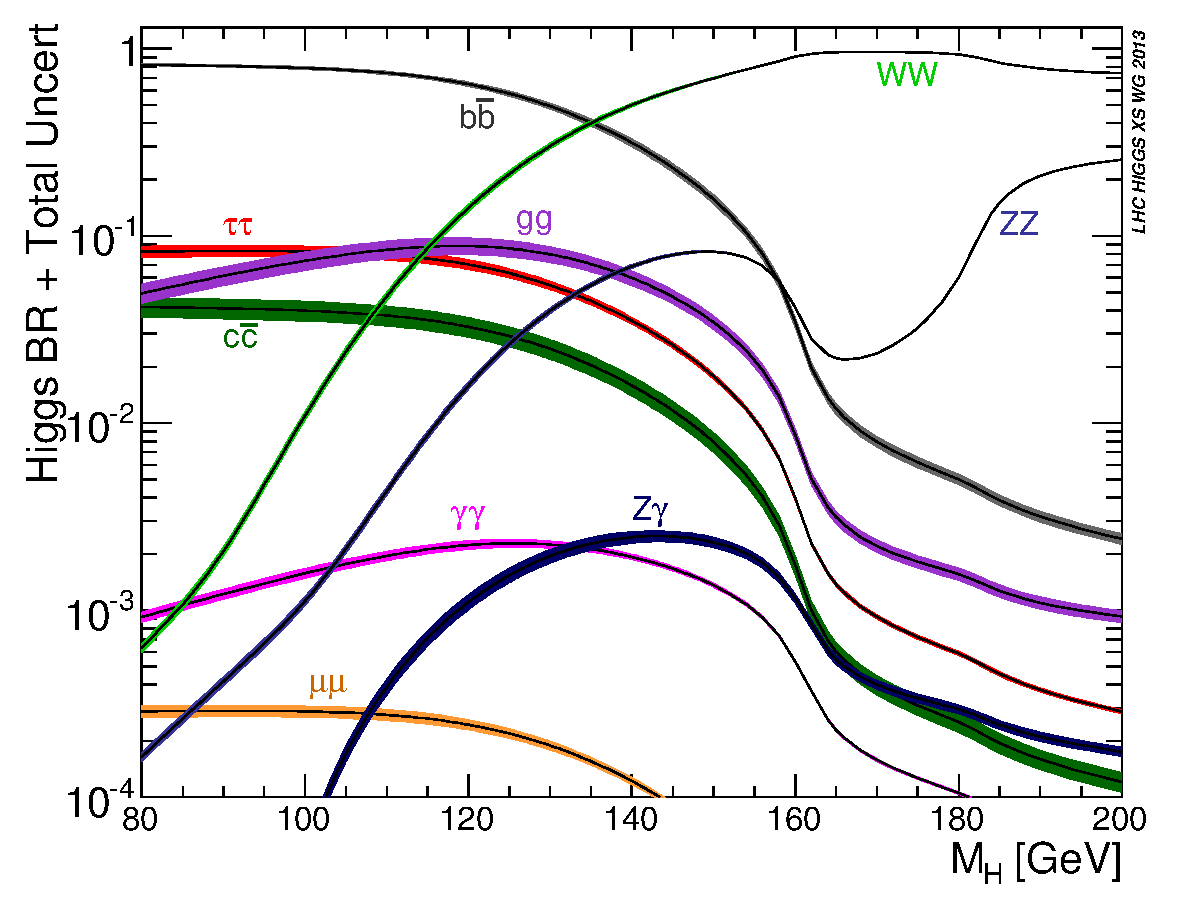
\includegraphics[width=0.90\textwidth]{Higgs_BR_LM_RECT}
    \caption[Higgs boson decay channels]{Higgs boson decay channels. At 125 GeV the dominant decay mode is $H \to b\bar{b}$.}
    \label{Higgs_BR_LM_RECT}
\end{figure}


Even though the facts above tell us about how great the SM is, SM is still far from being perfect. Masses of elementary particles are the parameters in this theory, they do not come from SM predictions. It is hypothesised that the SM could be a part of the larger ultimate theory, the so-called "The Theory of Everything" (TOE), which is to be written (had been a lifelong journey of another genius, Einstein \cite{aps_einstein}). There is hope that the TOE will be able to explain many phenomena, such as the quark mass hierarchy, flavor mixing, etc. Also, in the SM all neutrinos are massless, however, it has been shown that they have a non-zero mass \cite{Bilenky:2014ema}. This fact is one of the main motivations for theorists to look for extensions of the SM. 



